\documentclass[10pt,twocolumn,letterpaper]{article}

\usepackage{dependable_dnn}
\usepackage{times}
\usepackage{epsfig}
\usepackage{graphicx}
\usepackage{amsmath}
\usepackage{amssymb}
\usepackage{subfigure}
\usepackage[table, dvipsnames]{xcolor}

% Include other packages here, before hyperref.

% If you comment hyperref and then uncomment it, you should delete
% egpaper.aux before re-running latex.  (Or just hit 'q' on the first latex
% run, let it finish, and you should be clear).
\usepackage[pagebackref=true,breaklinks=true,letterpaper=true,colorlinks,bookmarks=false]{hyperref}

\iccvfinalcopy % *** Uncomment this line for the final submission

\def\iccvPaperID{} % *** Enter the Paper ID here
\def\httilde{\mbox{\tt\raisebox{-.5ex}{\symbol{126}}}}

% Pages are numbered in submission mode, and unnumbered in camera-ready
\ificcvfinal\pagestyle{empty}\fi

\begin{document}

%%%%%%%%% TITLE - PLEASE UPDATE
\title{Co-teaching: Robust Training of Deep Neural Networks with Extremely Noisy Labels \\ {\rm {\normalsize Seungmin Lee (profile2697@gmail.com; 2013-11420), Dept. of Computer Science and Engineering, Seoul National University}}} 

\maketitle
\thispagestyle{empty}

%%%%%%%%% BODY TEXT - ENTER YOUR RESPONSE BELOW

%%%%%%%%%%%%%%%%%
%%%%%%%%%%%%%%%%%
\section{Introduction}
This paper addresses training with extremely noisy labels. A network often fails to learn a task when labels are noisy. This phenomenon occurs because the network tries to memorize these noisy labels and fails to generalize. Meanwhile, recent studies on the memorization effects found that models first memorize clean examples and then memorize noisy ones. Based on these results, this paper tries to select clean examples out of the noisy examples and use them to update the network.

\section{Methods} 
The proposed method is simple. The method simultaneously trains two networks $f$ and $g$. While training, each network samples $r$\% examples from a minibatch in order of smallest loss. We denote those examples as $D_f$ and $D_g$, respectively. After selecting examples, the method updates the networks using co-teaching, which means updating the network $f$ using $D_g$ and the network $g$ using $D_f$. As the training step increases, the proposed method decays the sampling rate  $r$. This decaying is based on the results that models memorize clean examples first and then memorize noisy ones. If we do not decay $r$, the number of noisy examples sampled by models increases as the training step increases.

According to this paper, previous methods have inferiority of accumulated errors caused by the biased sample selection. More specifically, we can assume a model selects a noisy example as a clean example. Then, the error caused by the selection mistake infiltrates the model. Unfortunately, if once the model considers a noisy instance as a clean one, it is hard to remove the bias from the model. Therefore, as training proceeds, the more error is accumulated in the model. However, the proposed method appropriately disconnects accumulation by using two independent networks, as we can see in Figure~\ref{fig:error}.

 \begin{figure}[b]
	\centering
	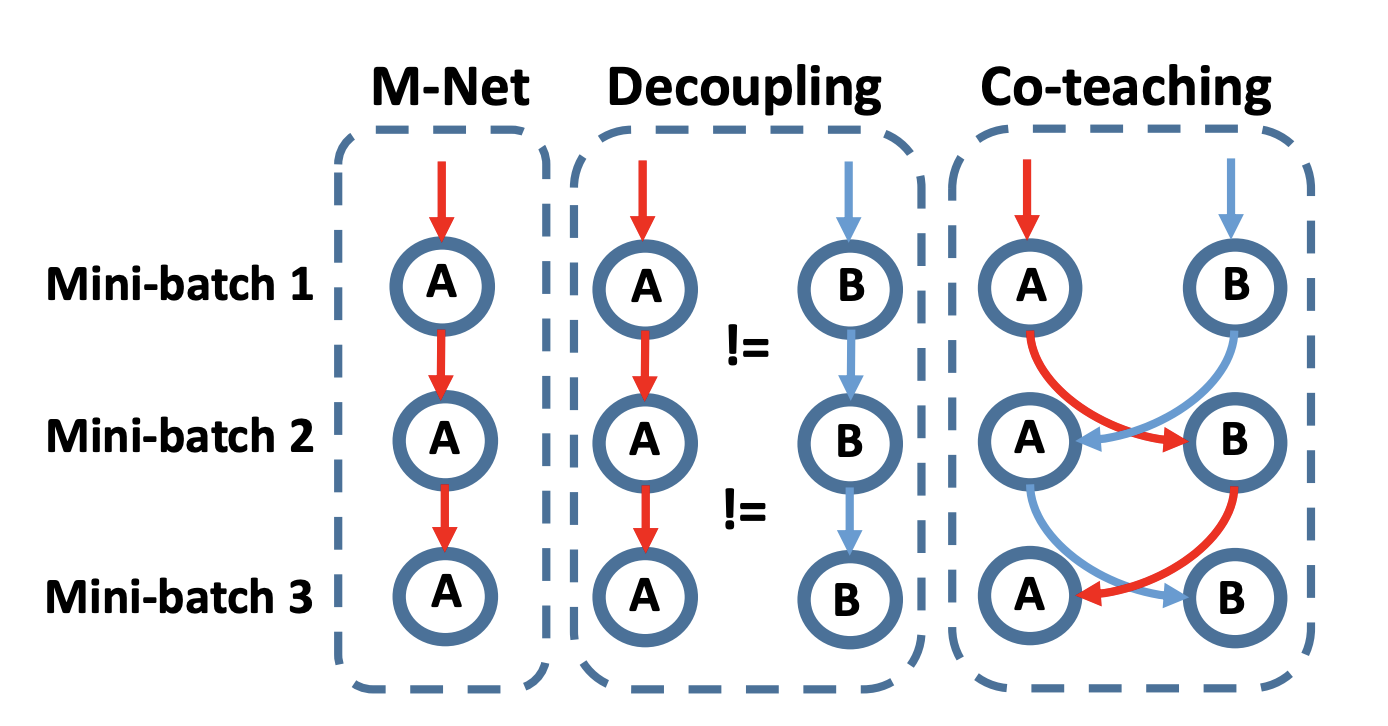
\includegraphics[width=6cm]{figures/coteaching.png}
	\caption{Comparison of error propagation.}
\end{figure}\label{fig:error}

%%%%%%%%%%%%%%%%%
\section{Results}
The proposed method's performance is far better than previous methods on both symmetric and pair flipping experiments. However, the most important assumption of this paper is that the method can effectively select clean examples. Thus, I think the plot of label precision by epochs is more important (Figure~\ref{fig:label}). The label precision is the ratio of real clean examples among the examples selected by the proposed method as clean ones. As we can see in the figure, the proposed method picks clean examples more reliably than other methods, especially on pair flipping which is regarded as harder settings.

 \begin{figure}[t]
	\centering
	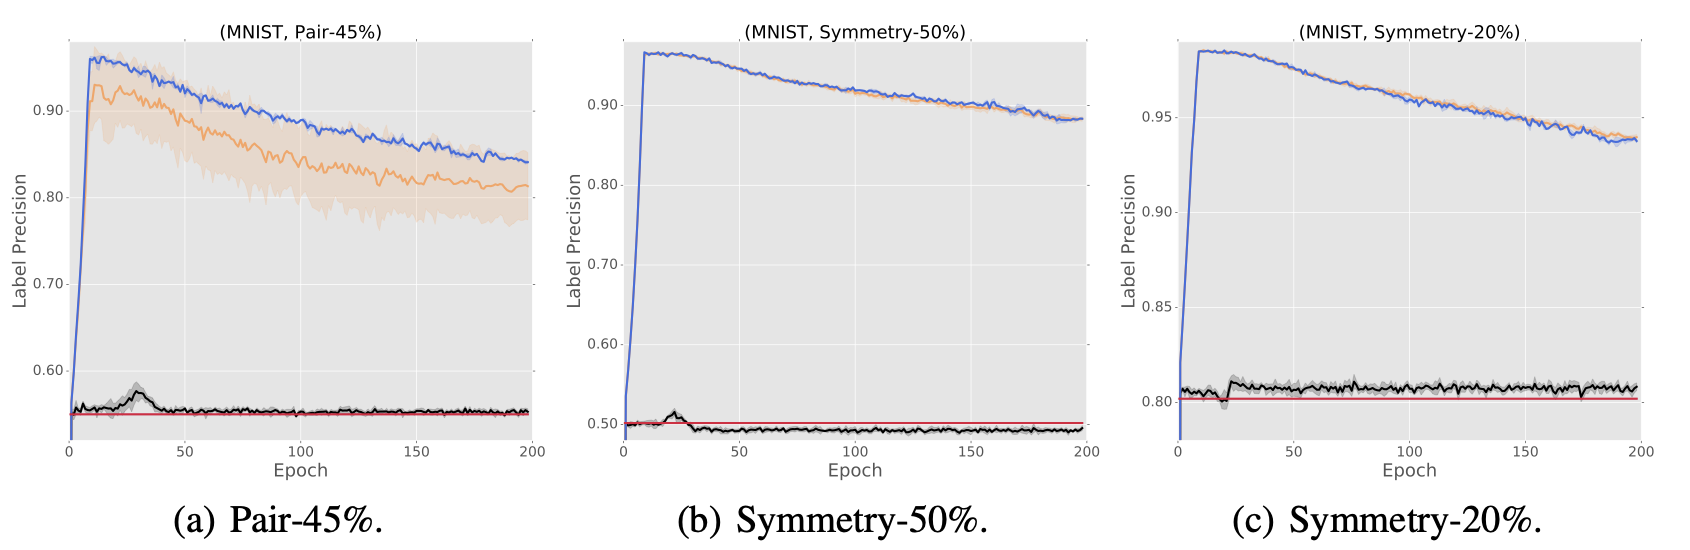
\includegraphics[width=8cm]{figures/labelprecision.png}
	\caption{Plot of label precision vs. epochs on MNIST.}
\end{figure}\label{fig:label}

\section{Personal Memo}
The proposed method seems simple and effective. It would be better if the figure included a plot of label precision without decaying $r$. Moreover, It would be better if I could see the results of other tasks because the method seems model-agnostic. Meanwhile, I wonder noisy labels can make decision boundary cross feature-dense regions. 

{\small
\bibliographystyle{ieee}
% \bibliography{egbib}
}

\end{document}
